% !TEX program = xelatex
\documentclass[12pt,letterpaper]{article}
\usepackage[margin=1in,headheight=15pt,headsep=.29in]{geometry}
\usepackage{fontspec}
\IfFontExistsTF{Times New Roman}{\setmainfont{Times New Roman}}{\setmainfont{Liberation Serif}}
\usepackage{babel}
\babelprovide[import,main]{spanish}
\usepackage{setspace,amsmath,amssymb,fancyhdr,booktabs,tabularx,array,tikz}
\usetikzlibrary{arrows.meta,positioning}
\usepackage{xurl}
\usepackage[hidelinks]{hyperref}
\hypersetup{pdftitle={Agente de optimización y autoescalado cloud (FinOps)},pdflang={es-CO}}
\urlstyle{same}
\fancypagestyle{apa}{
  \fancyhf{}
  \fancyhead[R]{\thepage}
  \renewcommand{\headrulewidth}{0pt}
  \renewcommand{\footrulewidth}{0pt}
}
\pagestyle{apa}
\doublespacing
\raggedright
\raggedbottom
\setlength{\parindent}{.5in}
\setlength{\parskip}{0pt}
\setlength{\emergencystretch}{2em}
\newcommand{\titulo}{Agente de optimización y autoescalado cloud (FinOps)}
\newcommand{\niveluno}[1]{\par\vspace{.35\baselineskip}\noindent\makebox[\linewidth][c]{\textbf{#1}}\par}
\newcommand{\niveldos}[1]{\par\vspace{.25\baselineskip}\noindent\textbf{#1}\par}
\newcommand{\entrada}[1]{\par\noindent\hangindent=.5in\hangafter=1 #1\par}
\newcolumntype{Y}{>{\raggedright\arraybackslash}X}
% Reemplace únicamente el texto entre llaves.
\newcommand{\Autores}{Larry David Botia Contreras}
\newcommand{\Afiliacion}{Programa de Ingeniería de Sistemas, Fundación Universitaria Los Libertadores}
\newcommand{\Curso}{IS0315 Technology Trends}
\newcommand{\Docente}{Gonzalo Rodríguez}
\newcommand{\FechaEntrega}{20 de noviembre de 2026}


\begin{document}
\vspace*{3\baselineskip}
\begin{center}
  \textbf{\titulo}\par\vspace{\baselineskip}
  \Autores\par
  \Afiliacion\par
  \Curso\par
  \Docente\par
  \FechaEntrega\par
\end{center}

\newpage
\niveluno{\titulo}
Una aplicación web pierde capacidad de respuesta si un pico de tráfico supera sus recursos. Mantener capacidad ociosa de forma permanente eleva el costo de operación. Este proyecto diseña y valida un agente de autoescalado que ajusta recursos cada minuto y considera el presupuesto antes de actuar. El prototipo aplica el enfoque de la guía (\textit{Taller de ingeniería de agentes inteligentes}, 2026) y refleja el propósito de FinOps de relacionar el costo con el valor operativo (FinOps Foundation, s. f.).

\niveluno{Modelo PEAS y propiedades del entorno}
\begin{samepage}
\noindent\textbf{Tabla 1}\par
\noindent\textit{Modelo PEAS del agente FinOps}\par
\begin{singlespace}
\small\setlength{\tabcolsep}{6pt}\renewcommand{\arraystretch}{1.20}
\noindent\begin{tabularx}{\linewidth}{@{}p{.21\linewidth}Y@{}}
\toprule
Componente & Aplicación en el laboratorio \\
\midrule
Performance & Disponibilidad por solicitudes $\geq 99{,}9\,\%$, latencia media $<200$ ms y menor gasto proyectado, sujeto al presupuesto de cada caso. \\
Environment & Tráfico variable, balanceador, clúster de contenedores sobre instancias web, base de datos gestionada y caché. El simulador representa la capacidad de esos componentes. \\
Actuators & Encender o apagar instancias web, aumentar un nivel de BD, activar o desactivar la caché y registrar alertas financieras u operativas. \\
Sensors & CPU, RAM y utilización de BD en porcentaje, latencia media en ms, solicitudes por segundo (RPS), disponibilidad por solicitudes, tarifas en USD/h, gasto acumulado, horas restantes y antigüedad de la lectura. \\
\bottomrule
\end{tabularx}
\end{singlespace}
\end{samepage}
\vspace{.35\baselineskip}

El entorno es \textbf{parcialmente observable}: las métricas agregadas ocultan la demanda futura y la proporción real de solicitudes cacheables. Es \textbf{no determinista desde la perspectiva operativa} porque el tráfico, los precios y los fallos pueden cambiar entre lecturas. Es \textbf{dinámico} y \textbf{secuencial}, pues cada acción altera el estado y el gasto futuro. Las decisiones se discretizan por minuto y las trazas de prueba son deterministas para facilitar su reproducción.

\newpage
\niveluno{Arquitectura del agente}

Un agente basado en utilidad permite comparar el estado futuro de varias configuraciones con una misma escala de decisión (Russell \& Norvig, 2021). Se eligió un modelo de transición explícito y auditable. El laboratorio emplea trazas sintéticas y parámetros fijos. La ventana de estabilización para reducir recursos toma como referencia el concepto documentado en Kubernetes (s. f.).

\noindent\textbf{Figura 1}\par
\noindent\textit{Flujo interno del agente de autoescalado}\par
\begingroup\centering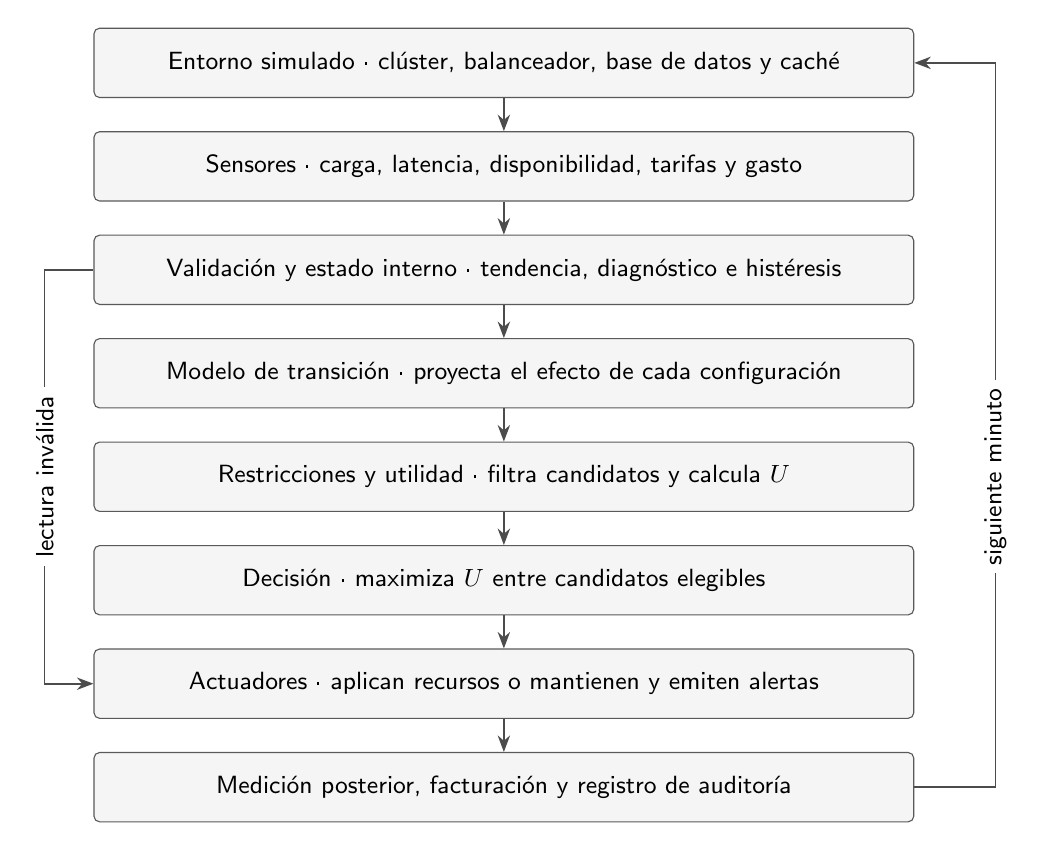
\begin{tikzpicture}[
  font=\small\sffamily,
  etapa/.style={draw=black!65, rounded corners=2pt, fill=black!4,
    align=center, text width=10.2cm, minimum height=8.8mm, inner sep=3pt},
  conex/.style={-{Stealth[length=2.1mm]}, line width=.6pt, draw=black!70},
  node distance=4.2mm]
\node[etapa] (entorno) {Entorno simulado · clúster, balanceador, base de datos y caché};
\node[etapa, below=of entorno] (sensores) {Sensores · carga, latencia, disponibilidad, tarifas y gasto};
\node[etapa, below=of sensores] (estado) {Validación y estado interno · tendencia, diagnóstico e histéresis};
\node[etapa, below=of estado] (modelo) {Modelo de transición · proyecta el efecto de cada configuración};
\node[etapa, below=of modelo] (utilidad) {Restricciones y utilidad · filtra candidatos y calcula $U$};
\node[etapa, below=of utilidad] (decision) {Decisión · maximiza $U$ entre candidatos elegibles};
\node[etapa, below=of decision] (actuadores) {Actuadores · aplican recursos o mantienen y emiten alertas};
\node[etapa, below=of actuadores] (traza) {Medición posterior, facturación y registro de auditoría};
\foreach \a/\b in {entorno/sensores,sensores/estado,estado/modelo,modelo/utilidad,
  utilidad/decision,decision/actuadores,actuadores/traza}
  \draw[conex] (\a) -- (\b);
\draw[conex] (estado.west) -- ++(-.62,0)
  |- (actuadores.west);
\node[rotate=90, fill=white, inner sep=3pt] at ([xshift=-.62cm]estado.west |- utilidad.west)
  {lectura inválida};
\draw[conex] (traza.east) -- ++(1.03,0) |- (entorno.east);
\node[rotate=90, fill=white, inner sep=3pt] at ([xshift=1.03cm]sensores.east |- utilidad.east)
  {siguiente minuto};
\end{tikzpicture}
\par\endgroup
\noindent\small\textit{Nota.} Una lectura inválida conserva los recursos y emite una alerta. El registro incluye las proyecciones y la observación posterior a la actuación.\par\normalsize

La clase \texttt{AgenteFinOps} conserva la tendencia de RPS, las muestras bajas y el último cambio. Si el simulador rechaza la configuración, conserva los recursos y registra el intento. El agente vuelve a evaluar con la siguiente lectura.

\newpage
\niveluno{Modelo de transición y presupuesto}

Sean $(n,d,b)$ las instancias web, niveles de BD y estado de caché actual ($b=0$ o $1$). Cada minuto se enumeran candidatos $s=(n',d',b')$ con entre 2 y 8 instancias, entre 1 y 3 niveles de BD, un descenso web máximo de 1, un aumento web máximo de 2 y un incremento de BD máximo de 1. La decisión usa la demanda actual $r$ y el promedio exponencial $\bar r_t=0{,}6r_t+0{,}4\bar r_{t-1}$, inicializado con la primera lectura válida.

Sea $D=\max(r,\bar r_t)$, $f=\max(1,\bar r_t/\max(r,1))$ y $g(b)=1-0{,}45b$. Sean $c,m,j$ las fracciones observadas de CPU, RAM y utilización de BD. La presión prevista del cuello de botella es el máximo de los cinco cocientes en la Ec. 1. El término de RAM descuenta un consumo fijo del 22\,\%.
\begin{equation}
 \rho(s)=\max\!\left\{\frac D{100n'},\;cf\frac n{n'},\;
 \frac{[m-0{,}22]_+}{0{,}78}f\frac n{n'},\;
 \frac{Dg(b')}{210d'},\;jf\frac d{d'}\frac{g(b')}{g(b)}\right\}.
\end{equation}

La notación $[x]_+=\max(x,0)$ indica la parte positiva. Con $\rho_0$ calculada para los recursos actuales usando $D=r$ y $f=1$, el residuo observado de latencia es $e_L=[L_{\mathrm{obs}}-55-95\rho_0^2]_+$. La latencia proyectada es $L(s)=55+95\rho(s)^2+e_L$ en milisegundos. La pérdida proyectada de solicitudes se aproxima con $p(x)=0{,}08\min(1,[x-0{,}85]_+)$ y la disponibilidad esperada es $A(s)=1-p(\rho(s))$. Son aproximaciones elegidas para comparar acciones.

El costo de cierre $C(s)$ extrapola el costo corriente durante las horas que quedan del mes. Con gasto acumulado $G$, horas restantes $H$ y tarifas por hora $t_w,t_d,t_b$, se usa
\begin{equation}
 C(s)=G+H\left(0{,}025+n' t_w+d' t_d+b't_b\right).
\end{equation}
El cargo fijo de USD 0,025/h corresponde al balanceador. Las tarifas iniciales son USD 0,075/h por instancia, USD 0,095/h por nivel de BD y USD 0,020/h por caché. Son supuestos de la simulación. El mes de referencia tiene 720 horas.

\newpage
\niveluno{Función de utilidad y restricciones}

Con presupuesto $B>0$, se define la utilidad adimensional en la Ec. 3. El beneficio por latencia se satura al llegar al objetivo, de modo que una reducción adicional no justifica por sí sola más gasto. El riesgo $R$ combina pérdida esperada en carga nominal (80\,\%) y en una situación con 15\,\% más presión (20\,\%). Cada pérdida se normaliza a partir del 2\,\% y se acota en 1.
\begin{align}
 U(s)&=0{,}30\min\!\left(1,\frac{200}{\max(L(s),1)}\right)
      -0{,}24\frac{C(s)}{B}-0{,}38R(s)-0{,}032M(s)-0{,}30E(s),\\
 R(s)&=0{,}8\min\!\left(1,\frac{p(\rho(s))}{0{,}02}\right)
      +0{,}2\min\!\left(1,\frac{p(1{,}15\rho(s))}{0{,}02}\right),\!
 \qquad E(s)=\left[\frac{C(s)}{B}-1\right]_+ .
\end{align}

$M$ es la suma de instancias web que cambian, un punto por cambiar BD y un punto por cambiar caché, dividida entre 4. Los pesos asignan la mayor penalización al riesgo. El costo penaliza el gasto relativo y el exceso añade presión para reducir una proyección que ya superó el presupuesto. El peso de cambio favorece estabilidad. Los pesos son parámetros de diseño, sin ajuste estadístico.

Una muestra inválida, repetida o con más de 90 s de antigüedad impide actuar. Reducir instancias o desactivar caché exige tres muestras válidas consecutivas con CPU, RAM y BD por debajo del 55\,\% y objetivos cumplidos. También exige tres minutos desde el último cambio y cumplimiento proyectado. Una acción que aumente el costo horario se bloquea si su cierre proyectado supera $B$. Mantener la configuración permanece disponible.

Entre candidatos permitidos se priorizan aquellos con $A\geq0{,}999$ y $L<200$ ms. El agente maximiza $U$ dentro de ese grupo o, si queda vacío, entre todos los permitidos y avisa. Los empates favorecen menos cambios y menor cierre. También se alerta al alcanzar el 90\,\% del presupuesto proyectado o al superar el 100\,\%.

En CP03-02, mantener dos instancias dio $U=-0{,}3077$ y 328,0 ms proyectados. Encender dos más dio $U=0{,}1279$ y 178,2 ms, con cierre de USD 370,80 ante un presupuesto de USD 570. La decisión aplicada fue ampliar a cuatro instancias.

\newpage
\niveluno{Diseño de pruebas}

Se ejecutaron once casos con y sin agente desde la misma configuración inicial y la misma secuencia de carga. El comparador fijo conserva los recursos de partida. Cada caso dura entre dos y siete minutos simulados. El entorno tiene capacidades efectivas distintas de las estimadas y puede variar la presión de la BD, la proporción cacheable o la latencia externa. Después de la decisión mide solicitudes ofrecidas y exitosas, latencia y costo del intervalo.

\noindent\textbf{Tabla 2}\par
\noindent\textit{Matriz de casos y conducta esperada}\par
\begin{singlespace}
\small\setlength{\tabcolsep}{5pt}\renewcommand{\arraystretch}{1.24}
\noindent\begin{tabularx}{\linewidth}{@{}p{.09\linewidth}p{.13\linewidth}>{\raggedright\arraybackslash}p{.30\linewidth}Y@{}}
\toprule
Caso & Tipo & Estímulo & Validación \\
\midrule
CP01 & Rutinario & 85--92 RPS. & Mantener recursos, sin alertas. \\
CP02 & Rutinario & 60--63 RPS y cuatro instancias. & Retirar una por ventana hasta llegar al mínimo. \\
CP03 & Crítico & Pico a 290--300 RPS con dos instancias. & Añadir dos instancias y recuperar la capacidad. \\
CP04 & Crítico & BD saturada con tráfico no cacheable. & Tras un intento ineficaz con caché, aumentar el nivel de BD. \\
CP05 & Crítico & 230 RPS con alto potencial de caché. & Activar caché sin aumentar el nivel de BD. \\
CP06 & Ambiguo & CPU ausente y muestra de 120~s. & Conservar recursos y registrar las dos causas. \\
CP07 & Crítico & 460 RPS y presupuesto de USD~210. & Bloquear expansiones fuera de presupuesto y avisar del compromiso. \\
CP08 & Ambiguo & Ráfagas y caídas alternas. & Evitar ciclos de encendido y apagado web. \\
CP09 & Crítico & Rechazo del primer cambio. & Conservar el estado, alertar y reevaluar en el siguiente intervalo. \\
CP10 & Crítico & Aumento tarifario con USD 370 consumidos. & Alertar por exceso proyectado y reducir capacidad cuando se habilite. \\
CP11 & Ambiguo & 300 ms externos con utilización baja. & Conservar recursos y alertar por el objetivo de latencia. \\
\bottomrule
\end{tabularx}
\end{singlespace}
\vspace{.35\baselineskip}

Las pruebas verifican decisiones, cambios reales de estado, alertas, restricciones y consistencia del máximo de utilidad. Las trazas JSONL conservan la telemetría, el puntaje y los bloqueos por candidato, la acción aplicada y el resultado posterior.

\newpage
\niveluno{Resultados de la simulación}

La disponibilidad observada es $100$ veces el cociente entre solicitudes exitosas y ofrecidas. La latencia media se pondera por el número de respuestas exitosas y el cumplimiento de latencia se cuenta por intervalo. Los SLA suelen expresar compromisos formales, mientras que los SLO fijan objetivos medibles (Jones et al., 2016). El 99,9\,\% se usa aquí como objetivo medido en cada traza. El costo facturado por minuto y el cierre mensual proyectado son indicadores distintos.

\noindent\textbf{Tabla 3}\par
\noindent\textit{Indicadores del agente y de la capacidad fija}\par
\begin{singlespace}
\small\setlength{\tabcolsep}{5pt}\renewcommand{\arraystretch}{1.25}
\noindent\begin{tabular*}{\linewidth}{@{\extracolsep{\fill}}lrrrrrrr@{}}
\toprule
 & \multicolumn{2}{c}{Disponibilidad (\%)} & \multicolumn{2}{c}{Latencia (ms)} & \multicolumn{2}{c}{Cierre (USD)} & $L<200$\\
\cmidrule(lr){2-3}\cmidrule(lr){4-5}\cmidrule(lr){6-7}
Caso & Agente & Fijo & Agente & Fijo & Agente & Fijo & Agente \\
\midrule
CP01 & 100{,}00 & 100{,}00 & 69{,}4 & 69{,}4 & 194{,}40 & 194{,}40 & 3/3 \\
CP02 & 100{,}00 & 100{,}00 & 58{,}5 & 58{,}2 & 194{,}41 & 302{,}40 & 7/7 \\
CP03 & 100{,}00 & 73{,}79 & 96{,}4 & 262{,}8 & 370{,}80 & 262{,}80 & 4/4 \\
CP04 & 96{,}89 & 90{,}68 & 111{,}6 & 187{,}2 & 385{,}20 & 302{,}40 & 3/3 \\
CP05 & 100{,}00 & 87{,}83 & 82{,}8 & 198{,}4 & 316{,}80 & 302{,}40 & 3/3 \\
CP06 & 74{,}81 & 74{,}81 & 264{,}3 & 264{,}3 & 248{,}40 & 248{,}40 & 0/2 \\
CP07 & 47{,}96 & 47{,}96 & 590{,}3 & 590{,}3 & 194{,}40 & 194{,}40 & 1/3 \\
CP08 & 100{,}00 & 100{,}00 & 76{,}1 & 103{,}5 & 262{,}80 & 248{,}40 & 6/6 \\
CP09 & 83{,}10 & 66{,}21 & 191{,}6 & 328{,}0 & 370{,}80 & 262{,}80 & 1/2 \\
CP10 & 100{,}00 & 100{,}00 & 57{,}9 & 57{,}9 & 398{,}60 & 406{,}19 & 4/4 \\
CP11 & 100{,}00 & 100{,}00 & 365{,}6 & 365{,}6 & 194{,}40 & 194{,}40 & 0/3 \\
\bottomrule

\end{tabular*}\par
\noindent\textit{Nota.} Cierre corresponde a la última proyección mensual. La columna final muestra los intervalos del agente bajo 200 ms sobre el total del caso.\par
\end{singlespace}

En CP02, las reducciones conservaron el 100\,\% de disponibilidad y disminuyeron el costo de siete minutos de USD 0,04900 a USD 0,04025 (17,86\,\%). En CP03, el agente obtuvo 100\,\% frente al 73,79\,\% de la capacidad fija y redujo la latencia media de 262,8 a 96,4 ms, con mayor cierre proyectado. En CP10, después del aumento de tarifa, la reducción de una instancia llevó el cierre previsto a USD 398,60 frente a USD 406,19 con capacidad fija y un límite de USD 400.

\newpage
\niveluno{Discusión y conclusiones}

Siete de las once trazas alcanzaron el objetivo de disponibilidad. Seis cumplieron también el umbral de latencia en todos sus intervalos. Los criterios de las trece pruebas se cumplieron, incluidos los que exigían observar una degradación o un bloqueo de seguridad. En CP07, el límite financiero impidió ampliar capacidad y la disponibilidad quedó en 47,96\,\%. El agente registró la necesidad de intervención mientras mantuvo el cierre proyectado en USD 194,40.

En CP04, la primera estimación sobrevaloró la eficacia de la caché. La ampliación de BD recuperó el servicio desde el siguiente intervalo, aunque la disponibilidad acumulada quedó en 96,89\,\%. En CP06, la falta de telemetría válida mantuvo la configuración sin corregir la saturación. En CP09, la acción aplicada en el segundo intervalo recuperó las solicitudes de ese minuto. CP11 mantuvo el 100\,\% de disponibilidad, con 365,6 ms de latencia media por la demora externa.

El agente muestra cómo responder a un pico sin sostener capacidad ociosa y cómo conservar presupuesto cuando el servicio tiene margen de reducción. Los resultados dependen de una simulación con cambios inmediatos, tarifas sintéticas, un horizonte corto y una estimación fija de caché. Las alertas quedan en registros locales. Una evaluación operativa necesitaría incorporar la tasa real de aciertos de caché, tiempos de aprovisionamiento, tarifas verificadas y ventanas representativas. La implantación comenzaría en modo sombra y avanzaría hacia cambios acotados tras comprobar los objetivos con telemetría del proveedor.

\niveldos{Reproducción}
El repositorio ejecuta las pruebas y guarda \texttt{metricas.csv}, \texttt{resumen.json} y \texttt{traza.jsonl} en \texttt{evidencia/}. En Windows se ejecuta \texttt{desplegar.cmd}. En macOS y Linux se ejecuta \texttt{sh desplegar.sh}. Se requiere Python 3.10 o posterior. La compilación del informe usa XeLaTeX y el diagrama se genera desde su fuente TikZ.

\newpage
\niveluno{Referencias}

\entrada{FinOps Foundation. (s. f.). \textit{FinOps framework}. \url{https://www.finops.org/framework/}}
\entrada{Jones, C., Wilkes, J., Murphy, N. R., \& Smith, C. (2016). Service level objectives. En B. Beyer, C. Jones, J. Petoff, \& N. R. Murphy (Eds.), \textit{Site reliability engineering: How Google runs production systems}. O’Reilly Media. \url{https://sre.google/sre-book/service-level-objectives/}}
\entrada{Kubernetes. (s. f.). \textit{Horizontal pod autoscaling}. \url{https://kubernetes.io/docs/concepts/workloads/autoscaling/horizontal-pod-autoscale/}}
\entrada{Russell, S. J., \& Norvig, P. (2021). \textit{Artificial intelligence: A modern approach} (4.ª ed.). Pearson.}
\entrada{\textit{Taller de ingeniería de agentes inteligentes: De los fundamentos a los sistemas multi-agente}. (2026, noviembre). [Guía de la actividad].}
\end{document}
